\chapter{LaTeX3 Token Lists}

 \TeX{} works with tokens, and \LaTeX3 therefore provides a number of
 functions to deal with lists of tokens.  Token lists may be present
 directly in the argument to a function:
 \begin{verbatim}
   \foo:n { a collection of \tokens }
 \end{verbatim}
 or may be stored in a so-called \enquote{token list variable}, which
 have the suffix \texttt{tl}: a token list variable can also be used as
 the argument to a function, for example
 \begin{verbatim}
   \foo:N \l_some_tl
 \end{verbatim}
 In both cases, functions are available to test an manipulate the lists
 of tokens, and these have the module prefix \texttt{tl}.
 
 
 In many cases, function which can be applied to token list variables
 are paired with similar functions for application to explicit lists
 of tokens: the two \enquote{views} of a token list are therefore collected
 together here.

 A token list (explicit, or stored in a variable) can be seen either
 as a list of \enquote{items},
 or a list of \enquote{tokens}. An item is whatever \docAuxCommand*{use:n} would
 grab as its argument: a single non-space token or a brace group,
 with optional leading explicit space characters (each item is thus
 itself a token list). A token is either a normal \texttt{N} argument,
 or \verb*| |, |{|, or |}| (assuming normal \TeX{} category codes).
 Thus for example
 \begin{verbatim}
   { Hello } ~ world
 \end{verbatim}
 contains six items (\texttt{Hello}, \texttt{w}, \texttt{o}, \texttt{r},
 \texttt{l} and \texttt{d}), but thirteen tokens (|{|, \texttt{H}, \texttt{e},
 \texttt{l}, \texttt{l}, \texttt{o}, |}|, \verb*| |, \texttt{w}, \texttt{o},
 \texttt{r}, \texttt{l} and \texttt{d}).
 Functions which act on items are often faster than their analogue acting
 directly on tokens.
%
% ^^A todo: perhaps move to another module, l3token or l3basics?
% \begin{texnote}
   When \TeX{} fetches an undelimited argument from the input stream,
   explicit character tokens with character code $32$ (space) and
   category code $10$ (space), which we here call \enquote{explicit
     space characters}, are ignored.  If the following token is an
   explicit character token with category code $1$ (begin-group) and an
   arbitrary character code, then \TeX{} scans ahead to obtain an equal
   number of explicit character tokens with category code $1$
   (begin-group) and $2$ (end-group), and the resulting list of tokens
   (with outer braces removed) becomes the argument.  Otherwise, a
   single token is taken as the argument for the macro: we call such
   single tokens \enquote{N-type}, as they are suitable to be used as
   an argument for a function with the signature~\texttt{:N}.

   When \TeX{} reads a character of category code $10$ for the first
   time, it is converted to an explicit space character, with character
   code $32$, regardless of the initial character code.
   \enquote{Funny} spaces with a different category code, can be
   produced using \docAuxCommand*{tl_to_lowercase:n} or \docAuxCommand*{tl\_to\_uppercase:n}.
   Explicit space characters are also produced as a result of
   \docAuxCommand*{token\_to\_str:N}, \docAuxCommand*{tl\_to\_str:n}, etc.
% \end{texnote}

 \section{Creating and initialising token list variables}

Before a token list can be used it needs to be created. It is important to recall that a token list is a \tex macro that holds tokens. This is achieved by using the e-\tex primitive \docAuxCommand*{unexpanded} inside a \tex |\edef| it is possible to store any tokens, including \#, in this way. The |\unexpanded| macro has been mapped to |\exp_not:n|.  This has made the token list registers (|\toks|) provided by \tex more or less redundant. Hence in |expl3| there are no |toks| registers.

 \begin{docCommand}{tl_new:N}{\meta{tl~var}}
    Creates a new \meta{tl~var} or raises an error if the
   name is already taken. The declaration is global. The
   \meta{tl~var} will initially be empty.
\end{docCommand}

In Example~\ref{ex:tl1}, line~\ref{lin:newlist} we will first create a new token list variable and then examine its meaning.
To examine its meaning, we use another |expl3| module function |\token_to_meaning:N|. This is the \tex primitive camouflaged in the new lingua. As we can see from the example a \meta{token list} is just a macro. 

\begin{texexample}{Create a token list variable}{ex:tl1}
\ExplSyntaxOn
% create the token list (*@\label{lin:newlist}@*)
\tl_new:N \g_mymodule_tl 

% examine its meaning
\token_to_meaning:N \g_mymodule_tl
\ExplSyntaxOff
\end{texexample}

If you have a basic knowledge of \tex programming, sometimes just peeking at the meaning of a function can give you a good understanding of what is happenning behind the scenes. In many of the example, I have included a line or two of code to examine the meaning of commands.


 \section{Adding data to token list variables}

Data can be added to the token list variable, as a once operation or added at left or right of the token list. The list can also be let to another one or emptied.

 \begin{docCommand}{tl_set:Nn}{\meta{tl~var} \marg{tokens}}
   Sets \meta{tl~var} to contain \meta{tokens},
   removing any previous content from the variable. The global |\tl_gset:Nn|, as well as different signature combinations are availabel such as \texttt{NV,Nv,No,Nf,Nx,cn,cV,cv,co,cf,cx}.
 \end{docCommand}

\begin{texexample}{Adding data}{ex:tl2}
\ExplSyntaxOn
% add something to the list
\tl_gput_left:Nn \g_mymodule_tl {This~is~something}
\token_to_meaning:N \tl_put_left:Nn
\ExplSyntaxOff
\end{texexample}

Let us put some more material and then view it again. This time we will add both to the left, as well as the right of the token list.

\begin{texexample}{Adding data}{ex:tl3}
\ExplSyntaxOn
% add something to the list
\tl_gput_left:Nn \g_mymodule_tl {LEFT~MATERIAL~}
\tl_gput_right:Nn \g_mymodule_tl {~RIGHT~MATERIAL}
\tl_gput_left:Nn \g_mymodule_tl {\bfseries}

% Use the token list
\g_mymodule_tl\\

% Another way to use it
\tl_use:N \g_mymodule_tl
\ExplSyntaxOff
\end{texexample}

The above are not the best of examples, but they illustrate the concepts well.

\begin{docCommand} {tl_put_left:Nn} {\meta{tl var} \marg{tokens}}
Prepends \meta{tokens} to the left side of the current content of \meta{tlvar}
\end{docCommand}

\begin{docCommand} {tl_put_right:Nn} {\meta{tl var} \marg{tokens}}
Appends \meta{tokens} to the right side of the current content of \meta{tlvar}
\end{docCommand}

\begin{texexample}{Append and prepend functions}{ex:prepend}
\ExplSyntaxOn
\tl_new:N  \phd_tempa_tl
\tl_new:N  \phd_tempb_tl
\tl_new:N  \phd_tempc_tl

\tl_put_left:Nn \phd_tempa_tl {First}
\tl_put_left:Nn \phd_tempa_tl {\bgroup\bfseries}
\tl_put_right:Nn \phd_tempa_tl {~Second\egroup}

\tl_set:Nn \phd_tempb_tl {\fbox{\tl_use:N \phd_tempa_tl }}

\tl_use:N \phd_tempb_tl

\tl_put_left:Nn \phd_tempb_tl { \fboxsep=3pt \fboxrule=0.1pt }

\tl_use:N \phd_tempb_tl

\phd_tempb_tl
\ExplSyntaxOff
\end{texexample}

The token list can be used simply by typing |\phd_tempb_tl| or by using the |\tl_use:N| function for example  |\tl_use:N \phd_tempb_tl|. The latter is preferred as it checks for naming errors. If for example the list name was mistyped it will give a |bad variable error|. It is also a good programming pattern to use, as it follows logically to \emph{construct} the list, \emph{manipulate} it and then \emph{use} it,  to typeset the contents. 



\subsection{Concatenation}

Two lists can be concatenated together by using a third list and adding the contents of the other two together.

\begin{texexample}{Concatenation and other functions}{ex:concat}
\ExplSyntaxOn
\tl_new:N  \tl_phd_temp_a
\tl_new:N  \tl_phd_temp_b
\tl_new:N  \tl_phd_temp_c
%%\tl_concat:NNN \tl_phd_temp_a \tl_phd_temp_b \tl_phd_temp_c
\ExplSyntaxOff
\end{texexample}


\begin{texexample}{Concatenation and other function}{ex:concat}
\ExplSyntaxOn
\cs_new:Nn\whatever:n{[{#1}]}

\cs_set:Nn\l_phd_test_helper: {
       \tl_set:Nn  \tl_phd_temp_a {Yiannis Mary John}
       \tl_put_left:Nn \tl_phd_temp_a {Dr.~}
       \tl_set:Nn  \tl_phd_temp_b {{Lazarides}{Lou}{Smith}}
       \tl_concat:NNN \tl_phd_temp_c \tl_phd_temp_a \tl_phd_temp_b
       \tl_map_inline:Nn\tl_phd_temp_c{\whatever:n{##1}}
}
\DeclareDocumentCommand\Test{ }
    {
      \l_phd_test_helper:
    }   
\ExplSyntaxOff 
\Test
\end{texexample}

The syntax of the concatenation function is shown below.

 \begin{docCommand}{ tl_concat:NNN}{ \meta{tl~var1} \meta{tl~var2} \meta{tl~var3}}
   Concatenates the content of \meta{tl~var2} and \meta{tl~var3}
   together and saves the result in \meta{tl~var1}. The \meta{tl~var2}
   will be placed at the left side of the new token list.
\end{docCommand}


 \begin{docCommand}{tl_const:Nn}{\meta{tl~var} \marg{token list}}
   Creates a new constant \meta{tl~var} or raises an error
   if the name is already taken. The value of the
   \meta{tl~var} will be set globally to the
   \meta{token list}.
 \end{docCommand}




\begin{texexample}{Concatenation and other function}{ex:concat}
\ExplSyntaxOn
\tl_concat:NNN \tl_phd_temp_a \tl_phd_temp_b \tl_phd_temp_c
\ExplSyntaxOff
\end{texexample}

\subsection{Search and replace}

It is an amazing feat that the \latexe Team has managed to provide replacement routines. These so far have not found meaningful application but I have an idea which I am going to share it with you in a moment.

\begin{texexample}{Replacement}{ex:replacement}
\ExplSyntaxOn
\tl_set:Nn \tempa {This~is~the~LaTeXe~logo.~The~LaTeXe~logo.}
\tl_replace_once:Nnn \tempa {LaTeXe} {\latexe}
\tl_use:N \tempa\par
\tl_replace_all:Nnn \tempa {LaTeXe} {\latexe}
\tl_use:N \tempa\par
\ExplSyntaxOff
\end{texexample}


\begin{texexample}{Replacement}{ex:replacement}
\long\def\putimage#1]]{%
   \bgroup
   \fboxsep=3pt
   \fboxrule=1pt
   \fbox{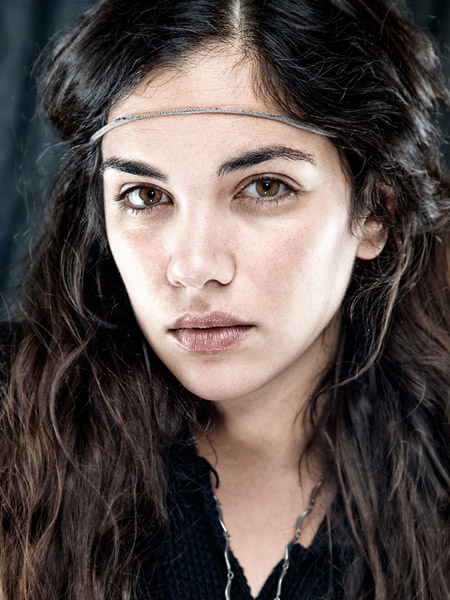
\includegraphics[width=3cm]{amato}}\hspace{2pt}%
   \egroup
}
\long\def\putsomecaption#1]]{
  \captionof{figure}{#1}
}

\ExplSyntaxOn
   \tl_set:Nn \tempai {
      \centering
      [[img amato]]
      [[cap This~is~the~first~caption]]
      [[img amato]]
      [[cap This~is~the~second~caption]]
      [[img amato.jpg]] 
      [[cap This~is~the~third~caption]]
   }
   \tl_replace_all:Nnn\tempai {[[img}{\putimage}
   \tl_replace_all:Nnn\tempai {[[cap}{\putsomecaption}
   \tl_use:N \tempai
\ExplSyntaxOff   
\end{texexample}

The code is still not mature and settled enough to provide an extensive search and replace, although a regex module has been coded by Bruno. However, simple templates can be developed such as the above. 

Of course in our first image example, we simplified the code in order to explain the concepts more clearly. In our second example we will add code so that the images are enclosed in a |minipage| and the captions set underneath the images. We will also center both the individual images as well as the three images overall.

\begin{texexample}{Replacement}{ex:replacement}
\long\def\putimage#1!!{%
    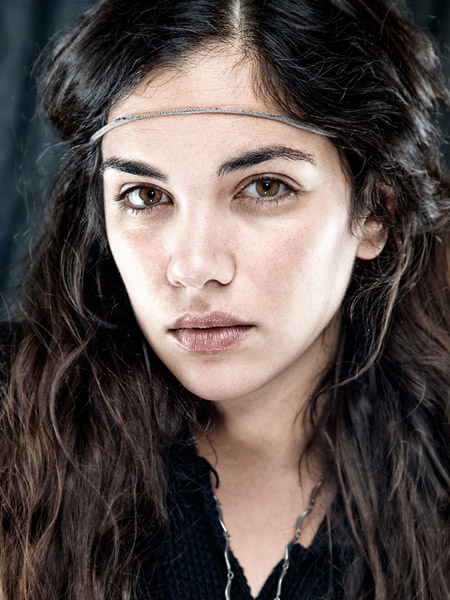
\includegraphics[width=\linewidth]{amato}%
 }
\long\def\putsomecaption#1!!{
  \captionof{figure}{#1}
  \par\endminipage\hfill
}


\ExplSyntaxOn
   \tl_set:Nn \tempai {
      \centering
      !!img amato!!
      !!cap This~is~the~first~caption!!
      
      !!img amato!!
      !!cap This~is~the~second~caption!!
      
      !!img amato.jpg!!
      !!cap This~is~the~third~caption!!
      
      !!img amato!!
      !!cap This~is~the~fourth~caption!!
      
      !!img amato!!
      !!cap This~is~the~fifth~caption!!
      
      !!img amato!!
      !!cap This~is~the~sixth~caption!!
 }
   \tl_replace_all:Nnn\tempai {!!img}{\minipage{3.6cm}\centering\putimage}
   \tl_replace_all:Nnn\tempai {!!cap}{\putsomecaption}
   \tl_use:N \tempai
\ExplSyntaxOff   
\end{texexample}

One might argue that by using |!!  !!| as a delimiter is not easier or clearer than say |\img |. In the final example I will propose another idea. But first let us create the environment. The best way to collect the body of the environment is to use the \pkgname{environ} package. 


When I posted the code at |TX.SX| egreg’s idea was to extend the code using a key value input and to be able to type:


\latex3 keys are discussed in the Chapter LaTeX3 key value and the example is reused but with key values. The second batch of images, shows some of the other challenges with the code. It will be best to have all the images measured and adjust the spacing in-between to be equal. 
\newpage


\ExplSyntaxOn
\NewEnviron{multiimages}[1][]
 {
  \keys_set:nn { yl/multiimages } { #1 }
  \tl_use:N \l_yl_multi_start_tl
  \dim_set:Nn \parindent { 0pt }
  \skip_set:Nn \leftskip { 0pt plus 1fil }
  \skip_set:Nn \rightskip { 0pt plus -1fil }
  \skip_set:Nn \lineskip { \l_yl_multi_skip_skip }
  \yl_multiimages:V \BODY
  \tl_use:N \l_yl_multi_end_tl
 }

\tl_new:N \l_yl_multi_start_tl
\tl_new:N \l_yl_multi_end_tl

\keys_define:nn { yl/multiimages }
 {
  env .choice:,
  env/none .code:n =
   \tl_set:Nn \l_yl_multi_start_tl { \par\addvspace{\topsep} }
   \tl_set:Nn \l_yl_multi_end_tl { \par\addvspace{\topsep} },
  env/figure .code:n =
   \tl_set:Nn \l_yl_multi_start_tl { \__yl_multi_beginfigure:V \l_yl_multi_pos_tl }
   \tl_set:Nn \l_yl_multi_end_tl { \end{figure} },
  env .initial:n = none,

  pos .tl_set:N = \l_yl_multi_pos_tl,
  pos .initial:n = { htp },

  outer .dim_set:N = \l_yl_multi_outer_dim,
  outer .initial:n = 3.6cm,
  inner .dim_set:N = \l_yl_multi_inner_dim,
  inner .initial:n = 3.6cm,

  skip .dim_set:N = \l_yl_multi_skip_skip,
  skip .initial:n = \lineskip,

  last .choice:,
  last/fill .code:n = 
   \tl_set:Nn \l_yl_multi_last_tl { { \parfillskip=0pt\par } },
  last/center .code:n =
   \tl_set:Nn \l_yl_multi_last_tl { { \parfillskip=0pt plus 2fil\par } },
  last .initial:n = fill,
 }

\cs_new_protected:Npn \__yl_multi_beginfigure:n #1
 {
  \begin{figure}[#1]
 }
\cs_generate_variant:Nn \__yl_multi_beginfigure:n { V }

\cs_new_protected:Npn \yl_multiimages:n #1
 {
  \tl_set:Nn \l_tmpa_tl { #1 }
  \tl_remove_all:Nn \l_tmpa_tl { \par }
  \tl_replace_all:Nnn \l_tmpa_tl { !!img ~ } { \__yl_multi_img:w }
  \tl_replace_all:Nnn \l_tmpa_tl { !!cap ~ } { \__yl_multi_cap:w }
  \tl_use:N \l_tmpa_tl \tl_use:N \l_yl_multi_last_tl
 }
\cs_generate_variant:Nn \yl_multiimages:n { V }

\cs_new_protected:Npn \__yl_multi_img:w #1 !!
 {
  \begin{minipage}{\l_yl_multi_outer_dim}\centering
  \includegraphics[width=\l_yl_multi_inner_dim]{ #1 }
 }
\cs_new_protected:Npn \__yl_multi_cap:w #1 !!
 {
  \captionof{figure}{#1}
  \end{minipage}\hspace{1pc plus 3pc}
 }
\ExplSyntaxOff   


\begin{multiimages}[last=center, env=figure,pos=ht]
  !!img 1975!! 
  !!cap This is the first caption!!

  !!img 1976!!
  !!cap This is the second caption!!

  !!img 1977!!
  !!cap This is the third caption!!

  !!img 1978!!
  !!cap This is the fourth caption!!

  !!img 1979!!
  !!cap This is the fifth caption!!

\end{multiimages}


\begin{multiimages}[last=center]
  !!img example-image-a!! 
  !!cap This is the first caption!!

  !!img example-image-a!!
  !!cap This is the second caption!!

  !!img example-image-a!!
  !!cap This is the third caption!!

  !!img example-image-a!!
  !!cap This is the fourth caption!!

  !!img example-image-a!!
  !!cap This is the fifth caption!!

\end{multiimages}

\begin{multiimages}[last=center,env=figure,pos=p,inner=3cm,skip=10ex]
  !!img example-image-a!! 
  !!cap This is the first caption!!

  !!img example-image-a!!
  !!cap This is the second caption!!

  !!img example-image-a!!
  !!cap This is the third caption!!

  !!img example-image-a!!
  !!cap This is the fourth caption!!

  !!img example-image-a!!
  !!cap This is the fifth caption!!

\end{multiimages}

\subsection{Token list conditionals}

The token list conditionals follow the same pattern than for other lists and are somewhat easier to remember.
There are conditional to check if the token list is empty, blank or equal to another. We just list the functions and provide an example at the end.

\begin{docCommand}{tl_if_blank:nTF}{\marg{token list} \marg{true code} \marg{false code}}
  Tests if the \meta{token list} consists only of blank spaces (i.e. contains no item). The test is
  true if \meta{token list} contains zero or more explicit space characters (explicit tokens with character
  code 32 and category code 10), and is false otherwise.
\end{docCommand}


\begin{texexample}{Token list conditionals}{ex:tlconditionals}
\ExplSyntaxOn
  \tl_set:Nn \l_tempa_tl {}
  \tl_if_blank:nTF \l_tempa_tl {\TRUE}{\FALSE}
\ExplSyntaxOff
\end{texexample}

\begin{docCommand}{tl_if_empty:NTF}{\marg{token list} \marg{true code} \marg{false code}}
  Tests if the \meta{token list variable} is entirely empty (i.e. contains no tokens at all). If the token list variable contains even a single space it returns false.
\end{docCommand}

\begin{texexample}{Token list conditionals}{ex:tlconditionals}
\ExplSyntaxOn
  \tl_set:Nn \l_tempa_tl { }
  \tl_if_empty:nTF \l_tempa_tl {\TRUE}{\FALSE}
  \tl_set:Nn \l_tempb_tl {}
  \tl_if_empty:nTF \l_tempb_tl {\TRUE}{\FALSE}
\ExplSyntaxOff
\end{texexample}

The |tl_case:NnTF| checks the token list variable against a series of one or more variables.

\begin{texexample}{Case}{tl}
\ExplSyntaxOn
\tl_set:Nn \l_tempa_tl {apple}
\tl_set:Nn \l_tempb_tl {apple}
\tl_set:Nn \l_tempc_tl {orange}

\tl_case:NnTF \l_tempa_tl
{
  { \l_tempb_tl }{is~apple~} 
  {\l_tempb_tl}{is~orange~}
}
{\TRUE}
{\FALSE}

\tl_set:Nn \l_tempb_tl {orange}

\tl_case:NnTF \l_tempc_tl
{
  { \l_tempb_tl }{is~orange~} 
  { \l_tempa_tl }{is~other~}
}
{\TRUE}
{\FALSE}

\ExplSyntaxOff
\end{texexample}

Another useful function tests if a token list var is in another token list. 



 